Dokažte, že neexistuje $\underset{x \rightarrow 0}{\lim} \sin\left(\frac{1}{x}\right)$.

\solution{
	Dokazujeme, že neexistuje limita.
	Zvolme tedy $\varepsilon = 1/2$ a chceme ukázat, že pro libovolné $\delta > 0$ existují $x_1, x_2 \in P(0, \delta)$ taková, že $|\sin(1/x_1) - \sin(1/x_2)| > 1/2$.
	Pro dané $\delta$ volíme $x_1 = \frac{1}{2 \pi \lceil \frac{1}{\delta} \rceil + \pi/2}$, $x_2 = \frac{1}{2 \pi \lceil \frac{1}{\delta} \rceil + 3\pi/2}$ (hodnoty sinu budou 1, -1).

	Viz Obrázek~\ref{fig:graf_sin_1_lomeno_x}.
	\begin{figure}[h]
		\centering
		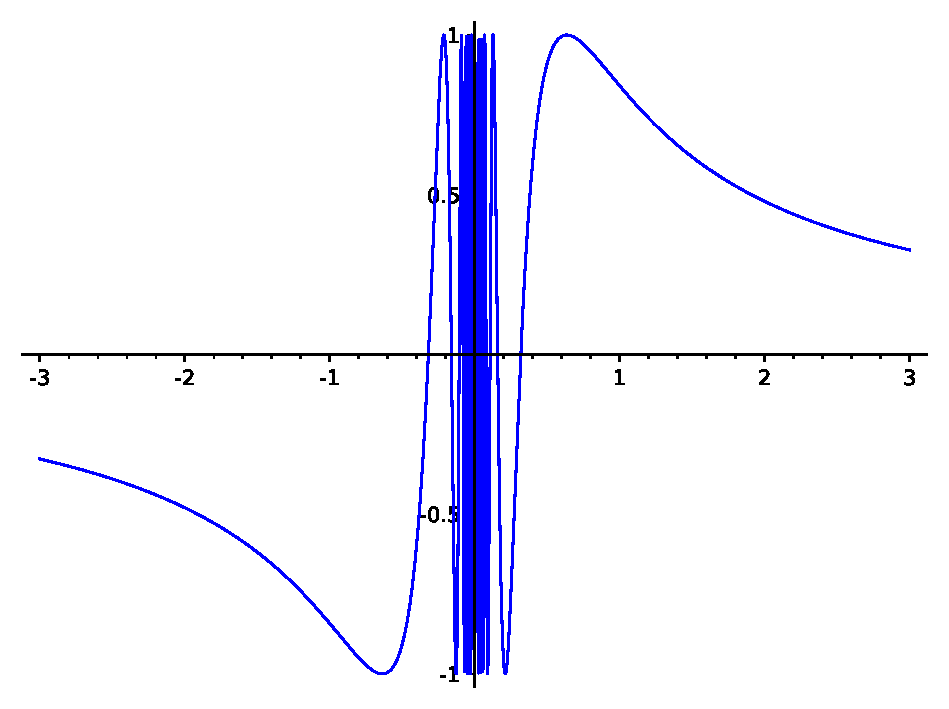
\includegraphics{cviceni_6/fig/sin_1_lomeno_x.pdf}
		\caption{$f(x) = \sin(1/x)$}
		\label{fig:graf_sin_1_lomeno_x}
	\end{figure}
}

